\documentclass[12pt,a4paper]{article}
\usepackage[slovene]{babel}
\usepackage[utf8]{inputenc}
\usepackage[T1]{fontenc}
\usepackage{lmodern}
\usepackage{microtype}
\usepackage{amsmath,amssymb,amsthm}
\usepackage{geometry}


\usepackage{tikz}


\DeclareMathOperator{\Int}{Int}
\theoremstyle{plain}
\newtheorem{definicija}{Definicija}[section]
\newtheorem{izrek}{Izrek}[section]



\title{ Interval index}
\author{Marija Mrvar in Jure Jerman \\ Projektna naloga}
\date{November 2025}



\begin{document}
\maketitle

\section{Uvod in definicije}


Naj bo $G = (V,E)$ končen, povezan in neusmerjen graf brez večkratnih povezav in zank.

\begin{definicija}
Za poljubni različni vozlišči $u, v \in V$ definiramo množico:
\[
I_G(u,v) = \bigl\{ w \in V \mid d_G(u,w) + d_G(w,v) = d_G(u,v) \bigr\}.
\]
Množica $I_G(u,v)$ vsebuje vsa vozlišča, ki ležijo na vsaj eni najkrajši $u$--$v$ poti v grafu $G$, vključno z vozliščema $u$ in $v$.
\end{definicija}


\begin{definicija}
Intervalni indeks grafa $G$ je definiran kot
\[
\Int(G) = \sum_{\substack{\{u,v\}\subset V}} \bigl( |I_G(u,v)| - 1 \bigr).
\]
\end{definicija}



Grafi, na katere se bomo osredotočili sta:
\begin{itemize}
    \item Pot $P_n$, ki je preprost povezan graf z $n$ vozlišči in $n-1$ povezavami, pri čemer so vozlišča urejena v zaporedju, tako da je vsako vozlišče (razen prvega in zadnjega) povezano z natanko dvema sosedoma
    \item Poln graf $K_n$, ki je preprost neusmerjen graf, v katerm je vsako
    vozlišče povezano z vsakim drugim vozliščem z natanko eno povezavo.
\end{itemize}


\section{Primera poti in polnega grafa}

\begin{center}
\vspace{3mm}
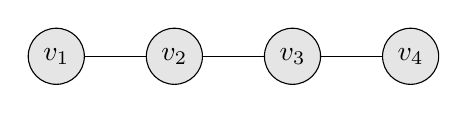
\begin{tikzpicture}[node distance=1.5cm, main/.style = {draw, circle, fill=gray!20, minimum size=6mm}]
    
    % Definicija vozlišč
    \node[main] (1) at (0,0) {$v_1$};
    \node[main] (2) [right of=1] {$v_2$};
    \node[main] (3) [right of=2] {$v_3$};
    \node[main] (4) [right of=3] {$v_4$};
    
    % Risanje povezav
    \draw (1) -- (2);
    \draw (2) -- (3);
    \draw (3) -- (4);
    
\end{tikzpicture}
\end{center}


\begin{center}
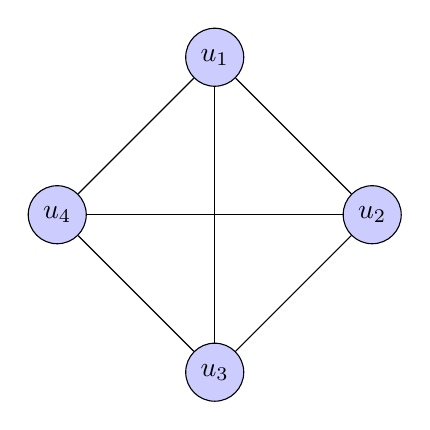
\begin{tikzpicture}[node distance=2cm, main/.style = {draw, circle, fill=blue!20, minimum size=6mm}]

    % Definicija vozlišč (postavljena v krog)
    \node[main] (A) at (90:2cm) {$u_1$};
    \node[main] (B) at (0:2cm) {$u_2$};
    \node[main] (C) at (-90:2cm) {$u_3$};
    \node[main] (D) at (180:2cm) {$u_4$};

    % Risanje vseh 6 povezav (vsako vozlišče z vsakim drugim)
    \draw (A) -- (B);
    \draw (B) -- (C);
    \draw (C) -- (D);
    \draw (D) -- (A);
    % Križne povezave
    \draw (A) -- (C);
    \draw (B) -- (D);
    
\end{tikzpicture}
\end{center}



\section{Cilji}

Najprej se bomo osredotočili na manjše grafe, potem pa sklepali na večje grafe, pri tem 
pa bomo predvsem želeli:


\begin{enumerate}
    \item Dokazati, da med vsemi grafi z $n$ vozlišči intervalni indeks $\Int(G)$ maksimizira pot $P_n$.
    \item Med vsemi povezanimi kubičnimi (3-regularnimi) grafi na $n$ vozliščih poiskati:
    \begin{itemize}
        \item graf z minimalno vrednostjo $\Int(G)$,
        \item graf z maksimalno vrednostjo $\Int(G)$,
    \end{itemize}
    ter opisati strukturne lastnosti teh ekstremalnih grafov (premer, število najkrajših poti, itd.).
\end{enumerate}




\end{document}
